\section{Audio Preprocessing}


Audio preprocessing is an essential step that is performed on audio data before it is fed into machine learning models. The objective of audio preprocessing is to clean the collected audio data, extract relevant features, and transform the data into a format that can be easily interpreted by the models. This section discusses important aspects of audio preprocessing, including noise reduction and audio trimming.


\subsection{Noise Reduction}

One of the key techniques used in audio preprocessing is noise reduction. In audio data, noise can arise from a variety of sources, such as background noise, microphone interference, or electrical interference. The presence of noise in the audio data can significantly impact the performance of the system, therefore it is i

One common strategy for denoising music is spectral gating, which involves gating the signal only on high-level sounds. Non-stationary noise reduction is an extension of stationary noise reduction that allows the noise gate to change over time. In this method, a spectrogram is calculated over the signal, and a time-smoothed version of the spectrogram is computed using an IIR filter applied forward and backward on each frequency channel. A mask is computed based on the time-smoothed spectrogram, which is then smoothed with a filter over frequency and time. The mask is applied to the spectrogram of the signal and then inverted.

To implement these noise reduction techniques, we recurred to the \textit{noisereduce} library. This algorithm relies on the spectral gating method and estimates a noise threshold for each frequency band of the signal/noise. This threshold is used to compute a mask, which gates noise below the frequency-varying threshold. The Code Snippet \ref{nr:code} shows how we implemented the noise reduction technique.

\begin{listing}[H]
	\begin{minted}{python}
noisereduce.reduce_noise(
	y=y, sr=16000, n_fft=2048, hop_length=512, prop_decrease=.75, time_constant_s=1
)
	\end{minted}
	\caption{Python code for applying noise reduction using the \textit{noisereduce} library.}
	\label{nr:code}
\end{listing}


\subsection{Audio Trim}

Another important aspect of audio preprocessing is audio trimming. This technique involves removing unwanted portions of the audio signal that are not relevant to the machine-learning model. For instance, in speech recognition, it is common to trim the silence from the beginning and end of an audio clip. This not only reduces the computational overhead but also makes the data more manageable.

We chose to define 30 decibels or lower as silence and removed any audio segments at the beginning and end of each audio file that fell below this threshold. This was done because 30 decibels is generally considered a very low level of noise, and is often used as a standard threshold for measuring background noise levels in quiet environments.

The table \ref{trim_durations} shows the original and after trim durations for all of the \ac{iemo} audio files. The table suggests the trimming process was effective in removing unwanted noise at the beginning and end of the audio files, which resulted in shorter durations overall. 


\begin{table}[H]
	\centering
	\caption{Audio Files' Original and After Trim Durations}
	\label{trim_durations}
	\begin{tabular}{lrr}
		\toprule
		Metric & Original Duration & After Trim Duration \\
		\midrule
		Minimum  		&  0.585 	&  0.256 \\
		Mean 			&  4.549  	&  4.065 \\
		Maximum 		& 34.139   	& 33.184 \\
		\bottomrule
	\end{tabular}
\end{table}



\subsection{Conclusion}

Figure \ref{fig:prep} compares the waveform, spectrogram, and power spectral density of the original and preprocessed audio file from the \ac{iemo} dataset. It can be observed the amplitudes of the preprocessed waveform are reduced and that there are more silent parts compared to the original. The preprocessed spectrogram shows a cleaner and clearer representation, with reduced dB values in some time frames. The preprocessed power spectral density contains lower values of dB/Hz compared to the original audio. In addition to these visual observations, we also listen to the resulting audio and manually denoted the noise reduction and clearer audio.

\begin{figure}[H]
	\centering
	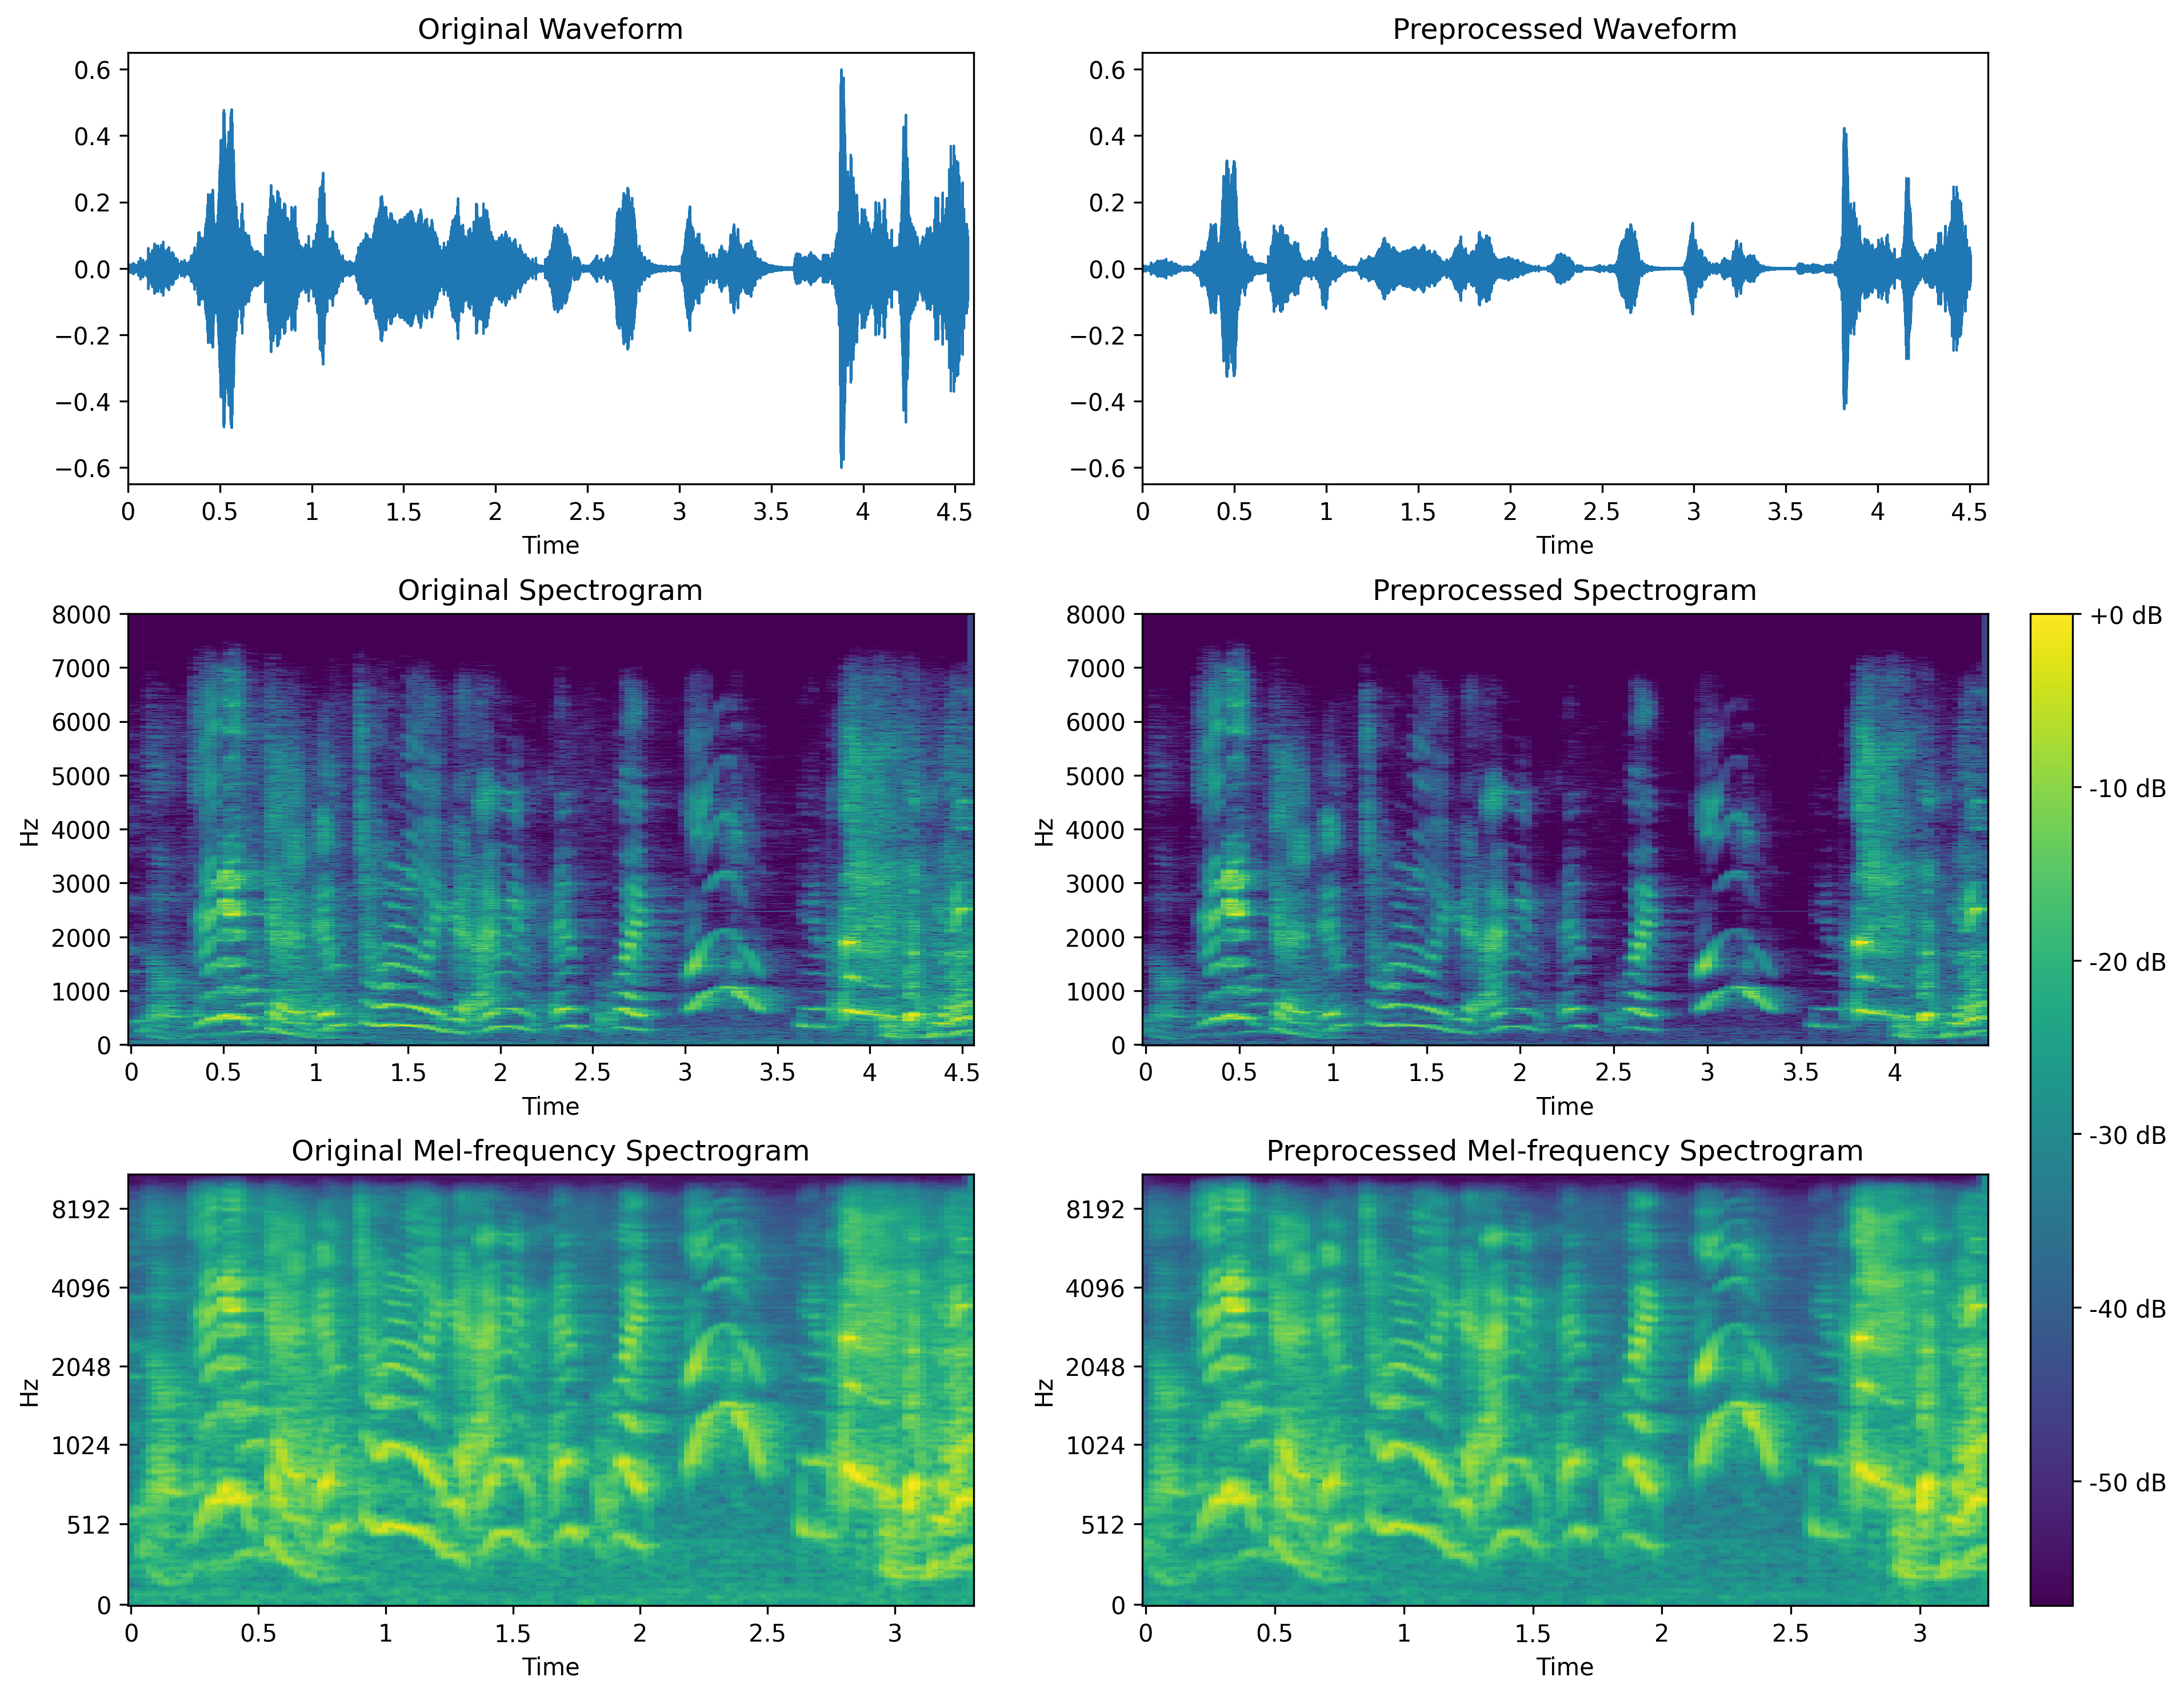
\includegraphics[width=\textwidth]{figs/4_2_preprocessing/preprocessing.png}
	\caption{Visual representations of audio features before and after preprocessing.}
	\label{fig:prep}
\end{figure}


These results showed that these techniques effectively cleaned the audio data, resulting in shorter durations and reducing the amount of noise. However, it is important to note that in some cases, noise may be part of the signal of interest, and removing it may lead to misinterpretation. Overall, audio preprocessing is essential to ensure the quality and accuracy of audio data, but it requires a deep understanding of audio signals to create an effective audio preprocessing pipeline.
